\documentclass[twoside]{article}
\usepackage{aistats2027}
\usepackage[round]{natbib}
\renewcommand{\bibname}{References}
\renewcommand{\bibsection}{\subsubsection*{\bibname}}
\usepackage{amsmath,amssymb,amsthm}
\usepackage{booktabs}
\usepackage{microtype}
\usepackage{graphicx}
\usepackage{xcolor}
\usepackage{url}
\usepackage{setspace}
% Tighten vertical spacing to fit in 8 pages
\setlength{\textfloatsep}{6pt plus 2pt minus 2pt}
\setlength{\floatsep}{6pt plus 2pt minus 2pt}
\setlength{\intextsep}{6pt plus 2pt minus 2pt}
\setlength{\abovecaptionskip}{4pt}
\setlength{\belowcaptionskip}{2pt}

\newcommand{\OSC}{\mathrm{OSC}}
\newcommand{\WS}{\mathrm{WS}}
\newcommand{\Heps}{\mathcal{H}_\varepsilon}
\newcommand{\Ddev}{\mathcal{D}_{\mathrm{dev}}}
\newcommand{\hhat}{\hat{h}}
\newcommand{\hstar}{h^*}
\newcommand{\Lval}{\hat{L}_{\mathrm{val}}}
\newcommand{\Ltest}{L_{\mathrm{test}}}
\newcommand{\bE}{\mathbb{E}}
\newcommand{\bP}{\mathbb{P}}

\runningtitle{How Certain Are We About the HPO Winner?}

\begin{document}

\twocolumn[

\aistatstitle{How Certain Are We About the HPO Winner?\\
Statistical Uncertainty in Hyperparameter Selection}

\aistatsauthor{ Anonymous Author(s) }
\aistatsaddress{ Anonymous Institution(s) }
]

%-----------------------------------------------------------------------
\begin{abstract}
We study uncertainty in hyperparameter selection rather than only
uncertainty in estimated model performance. We introduce
\emph{$\varepsilon$-optimal-set coverage} (OSC), which measures how
frequently bootstrap-resampled HPO runs select configurations whose
validation performance lies within $\varepsilon$ of the original winner.
OSC captures \emph{performance-space stability} and is conceptually
distinct from exact winner stability, which tracks whether the same
configuration is selected. Across seven datasets and three model
classes, OSC is negatively associated with post-selection
validation-to-test gaps (Spearman $r=-0.48$, 95\,\% CI
$[-0.59,-0.37]$), with consistent sign but heterogeneous magnitude
(forest-plot slopes all negative; $I^2=86\,\%$). In a paired
randomised experiment, replacing the HPO winner with a
stability-weighted selection reduces the post-selection gap, with
substantially larger benefits when OSC is low (decisive statistic
$\Delta\Delta G = +0.041$, $p < 0.001$; interaction
$\hat\beta_{\mathrm{Treatment}\times\mathrm{OSC}} = +0.075$, 95\,\%
bootstrap CI $[+0.051, +0.098]$). These results suggest that reliability
of HPO should be assessed in performance space rather than solely through
exact configuration stability.
\end{abstract}

%-----------------------------------------------------------------------
\section{Introduction}
\label{sec:intro}

Hyperparameter optimisation (HPO) is now a standard component of machine
learning pipelines. Given a model class and a development set, an HPO
procedure returns
\begin{equation}
  \hhat = \arg\min_{h \in \mathcal{H}} \Lval(h),
\end{equation}
and the associated validation loss $\Lval(\hhat)$ is reported as evidence
of the configuration's merit. This framing implicitly treats the identity
of $\hhat$ as unambiguous and its validation score as an unbiased
estimate of generalisation performance.

Neither assumption is warranted in general. Validation performance is
noisy: the development data is a finite random sample, and the
\emph{winner} of an HPO search is partly selected because it received a
favourable draw from this noise. The resulting discrepancy between
reported validation performance and subsequent test performance---the
\emph{post-selection gap} $G = \Ltest(\hhat) - \Lval(\hhat)$---is a
form of optimism bias well studied in model selection \citep{arlot2010survey,
cawley2010over,barnston1992long}. What is less studied is whether the
identity of $\hhat$ itself is reliable: for a given HPO procedure and
dataset, would a slightly different development sample have produced the
same winner?

We argue that this \emph{selection uncertainty} is a distinct and
practically important quantity. Two HPO runs can yield identical
validation scores but differ substantially in the stability of their
conclusions: one may consistently identify a narrow near-optimal region
regardless of which development sample is used, while the other
wanders across the search space and happens to win by chance. A practitioner
who cannot distinguish these situations cannot assess how much to trust
an HPO result.

Existing work on HPO focuses primarily on reducing the
\emph{number of function evaluations} required to find good configurations
\citep{snoek2012practical, li2018hyperband, falkner2018bohb,
bergstra2011algorithms}, or on providing confidence intervals for the
\emph{estimated performance} of a chosen configuration
\citep{dodge2019show, bouthillier2021accounting}. Stability
of the \emph{selection itself} has received comparatively little
attention, though related ideas appear in the stability selection
literature \citep{meinshausen2010stability} and in work on the
Rashomon set \citep{breiman2001random, semenova2022existence,
d2022underspecification}. Our contribution is to formalise this
distinction, provide a computable diagnostic, and demonstrate its
practical relevance.

\paragraph{Contributions.}
\begin{enumerate}\setlength\itemsep{2pt}
  \item We introduce \emph{$\varepsilon$-optimal-set coverage} (OSC), a
    bootstrap estimator of performance-space selection stability, and
    contrast it with exact winner stability (WS).
  \item We provide observational evidence across seven datasets that OSC
    predicts the post-selection gap independently of task, searcher,
    model class, and budget.
  \item We show experimentally that OSC moderates the benefit of
    stability-weighted selection: replacing the HPO winner with a
    centroid-based selection reduces post-selection gaps, with larger
    benefits when OSC is lower.
\end{enumerate}

%-----------------------------------------------------------------------
\section{Background and Related Work}
\label{sec:related}

\paragraph{Post-selection optimism.}
The gap between validation and test performance after model selection has
a long history in statistics \citep{tibshirani2009prediction}. In the
HPO setting, \citet{cawley2010over} showed that over-fitting to the
validation set is a serious concern when many configurations are evaluated.
\citet{dodge2019show} demonstrated that results reported from a single
HPO run are often poorly reproducible. Our work complements these by
asking not only \emph{how optimistic} a reported score is, but \emph{how
stable} the resulting configuration choice is.

\paragraph{Rashomon sets and model multiplicity.}
The Rashomon set $\mathcal{R}_\varepsilon = \{h : L(h) \le L(\hstar)+\varepsilon\}$
\citep{breiman2001random} contains all models that are nearly as good as
the best. Recent work \citep{semenova2022existence, marx2020predictive,
d2022underspecification} studies implications of a large Rashomon set.
OSC is complementary: the Rashomon set asks \emph{which configurations
are nearly optimal}; OSC asks \emph{whether the HPO procedure reliably
finds them}. High Rashomon-set size with low OSC signals a procedure
that fails to exploit a rich landscape of near-optimal configurations.

\paragraph{Stability selection.}
\citet{meinshausen2010stability} introduced stability selection for
feature selection, estimating the probability that each variable is
selected across bootstrap subsamples. Our bootstrap resampling strategy
is analogous, but we study stability of the \emph{configuration winner}
rather than of individual predictors, and we measure stability in
performance space rather than in the combinatorial space of variable sets.

\paragraph{HPO algorithm comparison.}
Extensive work compares HPO algorithms---random search, Bayesian
optimisation, successive halving, and their combinations
\citep{bergstra2012random, snoek2012practical, li2018hyperband,
falkner2018bohb}---primarily in terms of regret or final performance.
We contribute a complementary lens: for a fixed performance level, how
reliably does each algorithm identify the near-optimal region?

%-----------------------------------------------------------------------
\section{Method}
\label{sec:method}

\subsection{Setup and Notation}
\label{sec:setup}

Let $\mathcal{H}$ be a hyperparameter search space and
$\Ddev = \{(x_i, y_i)\}_{i=1}^n$ a development dataset. We randomly
partition $\Ddev$ into a training set $\mathcal{D}_\mathrm{tr}$ and a
validation set $\mathcal{D}_\mathrm{val}$, and maintain a separate
held-out test set $\mathcal{D}_\mathrm{test}$ that is never accessed
during HPO or OSC computation. An HPO procedure $\mathcal{A}$ searches
$\mathcal{H}$ and returns the \emph{winner}
$\hhat = \mathcal{A}(\mathcal{H}, \mathcal{D}_\mathrm{tr},
\mathcal{D}_\mathrm{val})$.

The \emph{post-selection gap} is
\begin{equation}
  G = \Ltest(\hhat) - \Lval(\hhat),
\end{equation}
where $\Lval(\hhat)$ is the validation loss used internally by $\mathcal{A}$
and $\Ltest(\hhat)$ is the loss on the held-out test set.
A positive $G$ indicates optimism: the procedure is more confident in
$\hhat$ than is warranted.

\subsection{Winner Stability and Its Limitations}
\label{sec:ws}

A natural stability diagnostic is \emph{winner stability} (WS): the
probability that the same configuration is re-selected under a perturbed
dataset. Using bootstrap resampling to approximate this, we draw $B$
resampled datasets $\mathcal{D}^{*(1)}, \ldots, \mathcal{D}^{*(B)}$,
rerun $\mathcal{A}$ on each, and estimate
\begin{equation}
  \WS = \frac{1}{B}\sum_{b=1}^{B}
    \mathbf{1}\bigl[\hhat^{(b)} \approx \hhat
    \text{ in } \ell_2\text{-config.\ space}\bigr].
\end{equation}

WS has a fundamental limitation: it measures stability in
\emph{configuration space}. In continuous search spaces, two
configurations can be far apart geometrically yet yield nearly identical
performance (e.g., in flat regions of the loss landscape). A procedure
that consistently selects configurations from the same near-optimal
region is reliable in the sense that matters for practitioners, even if
exact configuration identity varies across resamples. Conversely, a
procedure that repeatedly selects the same configuration can still be
unreliable if that configuration is a consistent noise artifact with
poor true performance.

Our empirical results confirm this: the expected post-selection gap is
essentially identical whether WS is high or low, conditional on OSC
(Table~\ref{tab:2x2}). WS does not predict $G$.

\subsection{$\varepsilon$-Optimal-Set Coverage}
\label{sec:osc}

We propose a stability measure defined in \emph{performance space}.
For a tolerance $\varepsilon > 0$, the $\varepsilon$-optimal set is
\begin{equation}
  \Heps = \bigl\{h : L(h) \le L(\hstar) + \varepsilon\bigr\},
\end{equation}
where $\hstar$ achieves the minimum of the true loss $L$. We approximate
membership in $\Heps$ using bootstrap validation losses. Let
$\hat{L}^{(b)}_\mathrm{val}$ denote the validation loss of the winner
$\hhat^{(b)}$ on the $b$-th bootstrap resample. We define
\begin{equation}
  \widehat{\OSC}_\varepsilon =
    \frac{1}{B}\sum_{b=1}^{B}
    \mathbf{1}\!\left[
      \hat{L}^{(b)}_\mathrm{val}(\hhat^{(b)}) \le
      \Lval(\hhat) + \varepsilon \cdot \widehat{\mathrm{range}}
    \right],
\label{eq:osc}
\end{equation}
where $\widehat{\mathrm{range}} = \max_b \hat{L}^{(b)}_\mathrm{val}
- \min_b \hat{L}^{(b)}_\mathrm{val}$ normalises $\varepsilon$ to the
scale of the observed loss distribution. We use $\varepsilon = 0.02$
throughout; Appendix~\ref{app:eps} shows robustness to this choice.

Intuitively, $\OSC$ measures the fraction of bootstrap-resampled HPO
runs whose winner achieves near-optimal performance on the corresponding
validation set. High OSC means the search reliably lands in the
near-optimal region across perturbations of the development data; low
OSC means the winner is sensitive to which data were observed, suggesting
a larger risk of post-selection disappointment.

\paragraph{OSC versus the Rashomon set.}
The Rashomon set characterises the landscape; OSC characterises the
procedure's ability to exploit it. A large Rashomon set together with
low OSC identifies a situation where near-optimal alternatives exist but
the search fails to find them consistently.

\paragraph{Computational cost.}
Computing OSC requires $B$ additional HPO runs. For cheap evaluation
budgets (e.g., tabular datasets with SVM or XGBoost), $B=30$--$50$
suffices and adds $B\times T_{\mathrm{run}}$ wall-clock time, where
$T_{\mathrm{run}}$ is the original HPO budget cost. All bootstrap runs
are parallelisable.

%-----------------------------------------------------------------------
\section{Experiments}
\label{sec:experiments}

\subsection{Setup}
\label{sec:setup_exp}

\paragraph{Datasets.} We use seven datasets spanning binary
classification, multiclass classification, and regression. Three
constitute the \emph{primary cohort} (breast\_cancer, wine, digits from
scikit-learn \citep{pedregosa2011scikit}); four constitute the
\emph{replication cohort} (diabetes regression, synthetic regression,
5-class multiclass, and a small high-variance binary dataset). Dataset
details are in Appendix~\ref{app:datasets}.

\paragraph{Model classes and search spaces.} We use three model
classes: (1) SVM-RBF with $(C, \gamma)$; (2) XGBoost with 5
hyperparameters; (3) MLP with 4 hyperparameters. Regression tasks use
SVR with $(C, \gamma, \varepsilon)$.

\paragraph{HPO algorithms.} We compare random search (RS), Bayesian
optimisation via TPE \citep{bergstra2011algorithms}, and successive
halving \citep{li2018hyperband} at evaluation budgets of 20 and 40.

\paragraph{Bootstrap.} We use $B=40$--$60$ bootstrap resamples for
the primary cohort and $B=25$--$50$ for the replication cohort. Each
resample resamples $\Ddev$ with replacement and re-splits into
train/val.

\paragraph{Reproducibility.} Code, all 378 observational runs, and all
180 intervention pairs are available at the anonymous repository linked
in the supplement.

\begin{figure}[t]
\centering
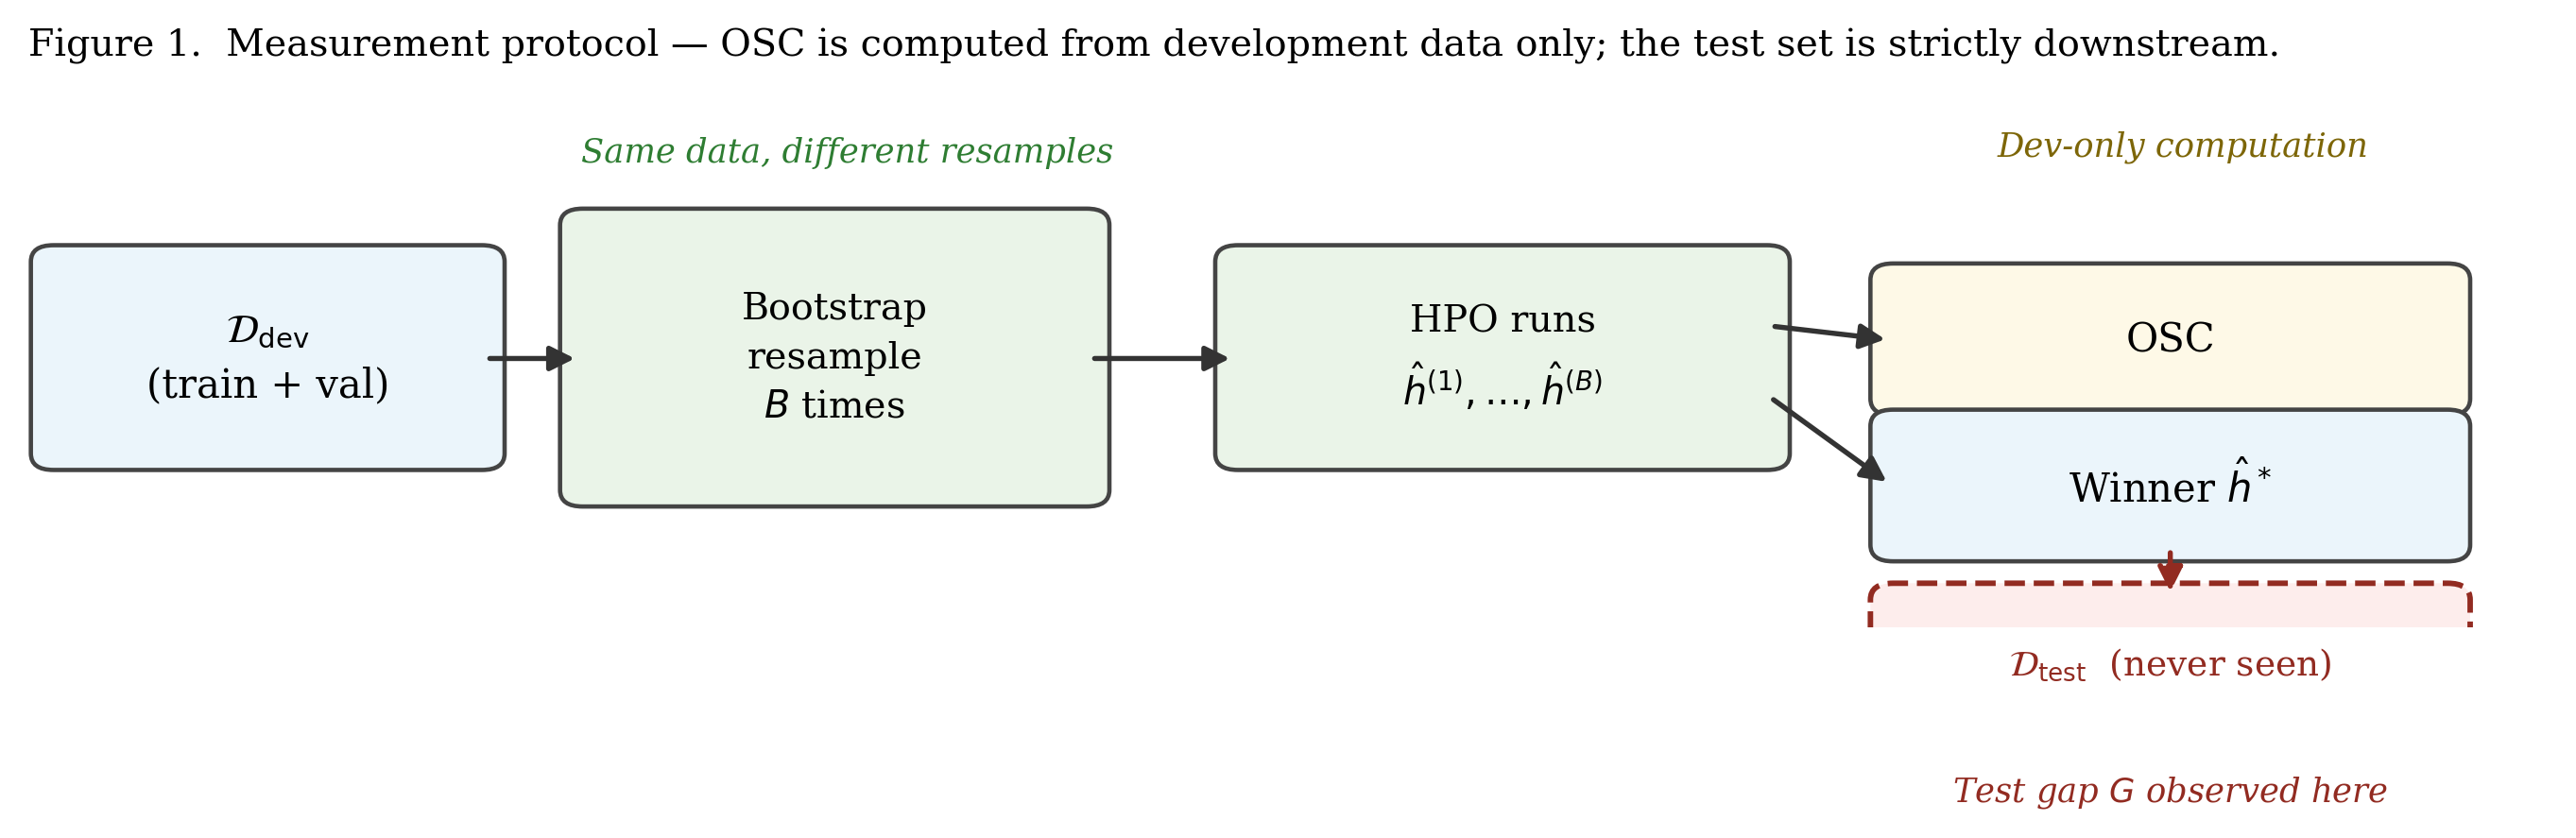
\includegraphics[width=0.97\columnwidth]{fig1_protocol.png}
\caption{Measurement protocol. OSC is computed from bootstrap resamples
of the development set (Steps 1--3) before any test evaluation
(Steps 4--5). The test set is strictly downstream.}
\label{fig:protocol}
\end{figure}

\subsection{Experiment 1: Observational Association}
\label{sec:obs}

We run each (dataset, model, searcher, budget, seed) combination and
record OSC, WS, and $G$. We then ask: does OSC predict $G$, after
controlling for covariates?

\begin{figure}[t]
\centering
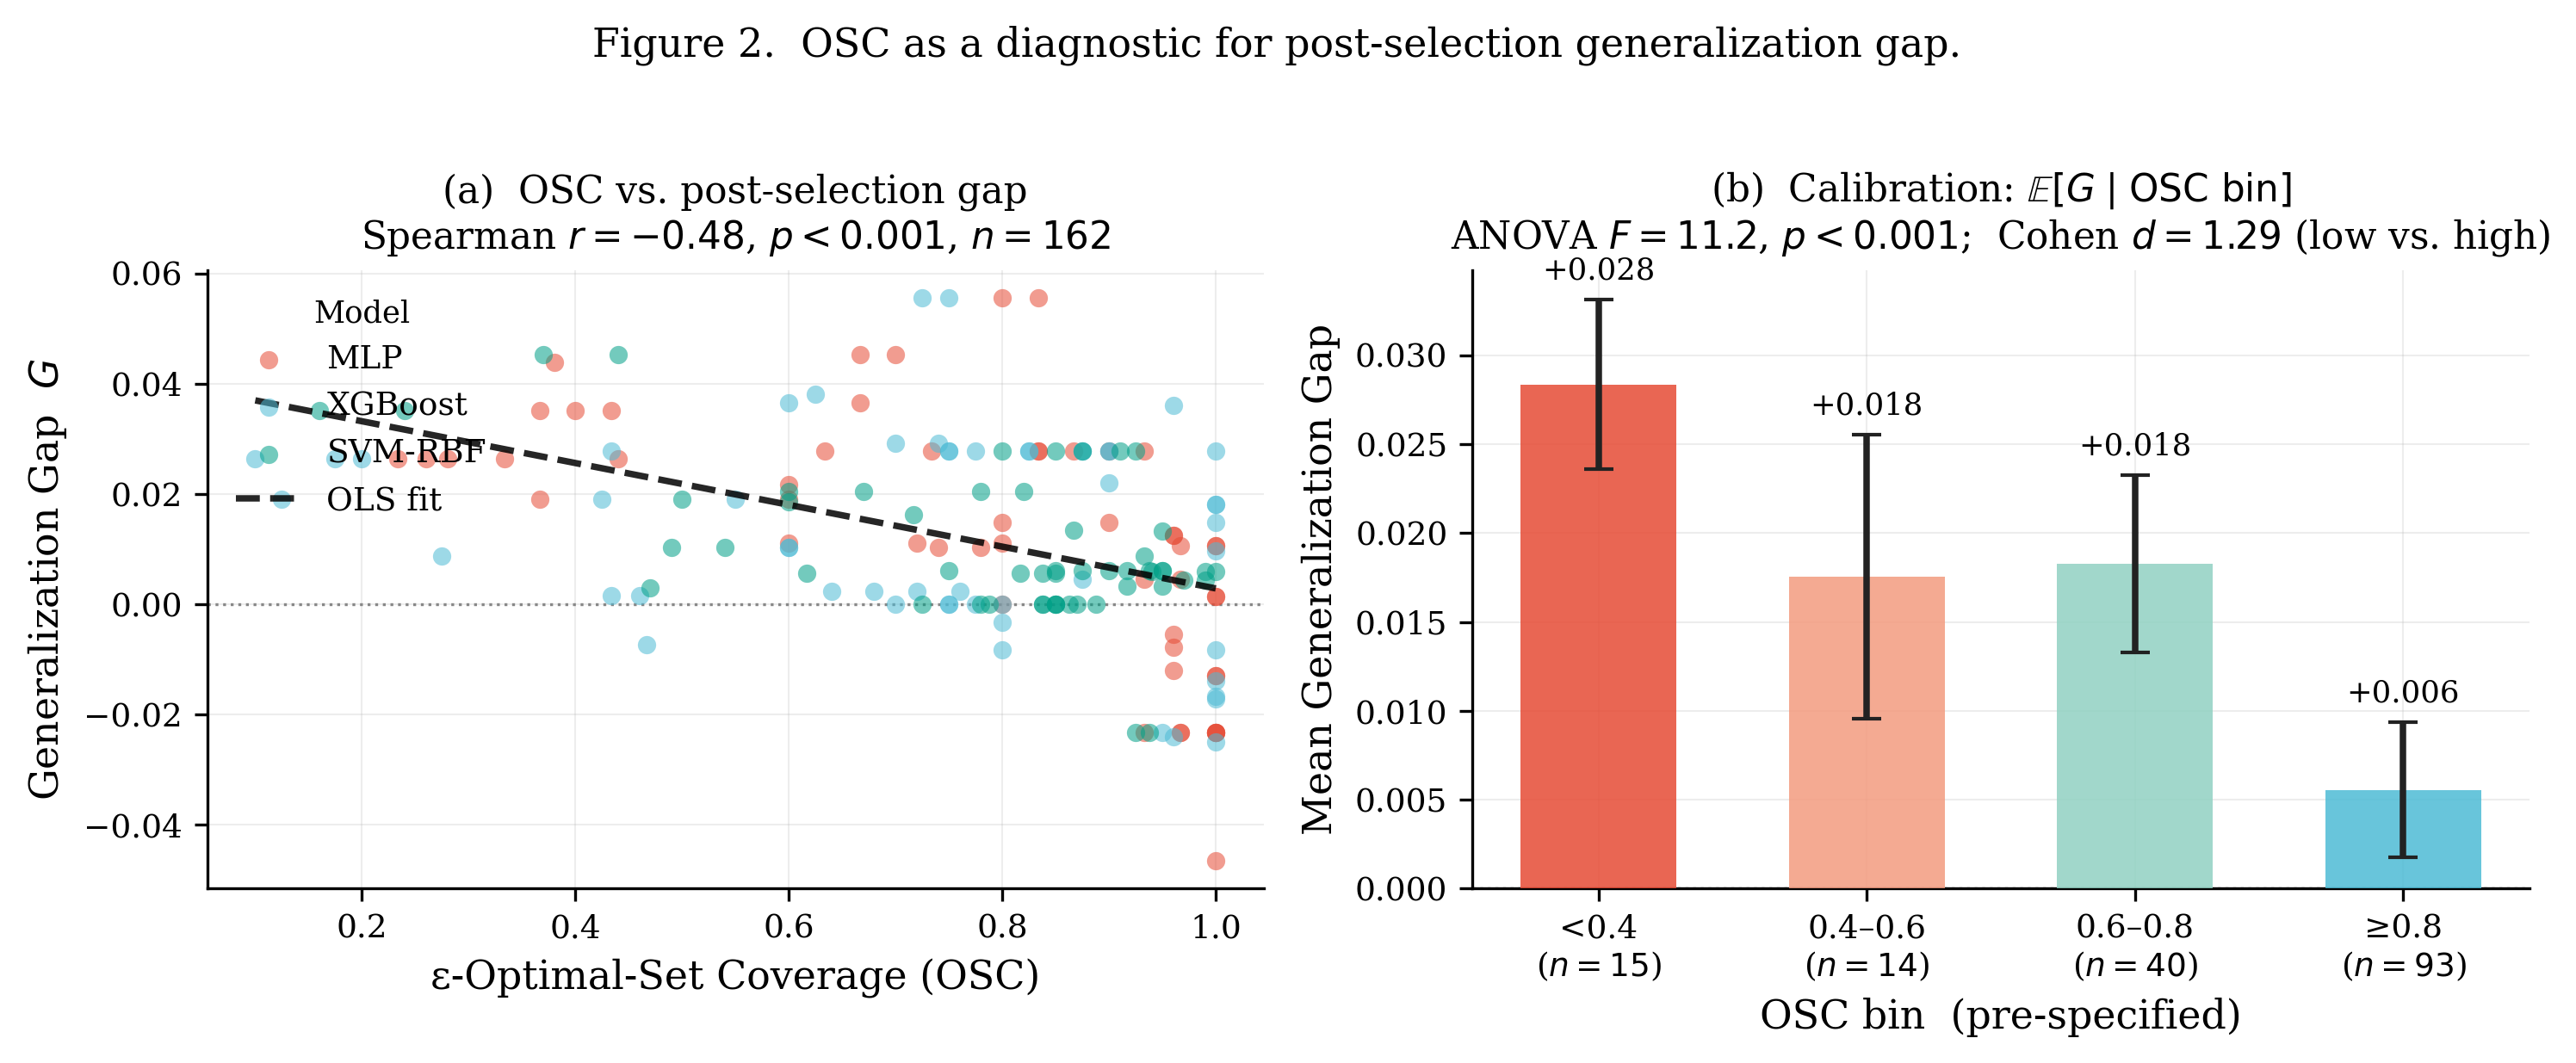
\includegraphics[width=0.97\columnwidth]{fig2_osc_vs_gap.png}
\caption{(a) OSC vs.\ post-selection gap, coloured by model class.
(b) Calibration: $\bE[G \mid \mathrm{OSC\ bin}]$ with 95\,\% CIs.
Bins are pre-specified; Cohen $d=1.29$ between low and high tails.}
\label{fig:calibration}
\end{figure}

\paragraph{Main result.}
Across 162 runs in the primary cohort, the Spearman correlation between
OSC and $G$ is $r = -0.48$, 95\,\% bootstrap CI $[-0.59, -0.37]$,
$p < 0.001$. In a controlled OLS regression
\begin{equation*}
  G \sim \OSC + \text{task} + \text{searcher} + \text{dataset} + \text{budget},
\end{equation*}
the OSC coefficient is $-0.029$ (SE $= 0.008$, $p = 0.0004$), with
partial $R^2 = 0.078$. A linear mixed-effects model with random intercept
per dataset gives $-0.035$ ($z = -4.13$, $p < 0.001$). The effect is
stable across five model specifications (Table~\ref{tab:osc_coef}).

By contrast, WS is not significantly associated with $G$
($r = -0.13$, 95\,\% CI $[-0.28, +0.03]$). The distinction is not
merely quantitative: the cross-classified 2$\times$2 table (OSC and WS
split at their medians) shows that high WS without high OSC provides no
protection against large gaps (Table~\ref{tab:2x2}).

\begin{figure}[t]
\centering
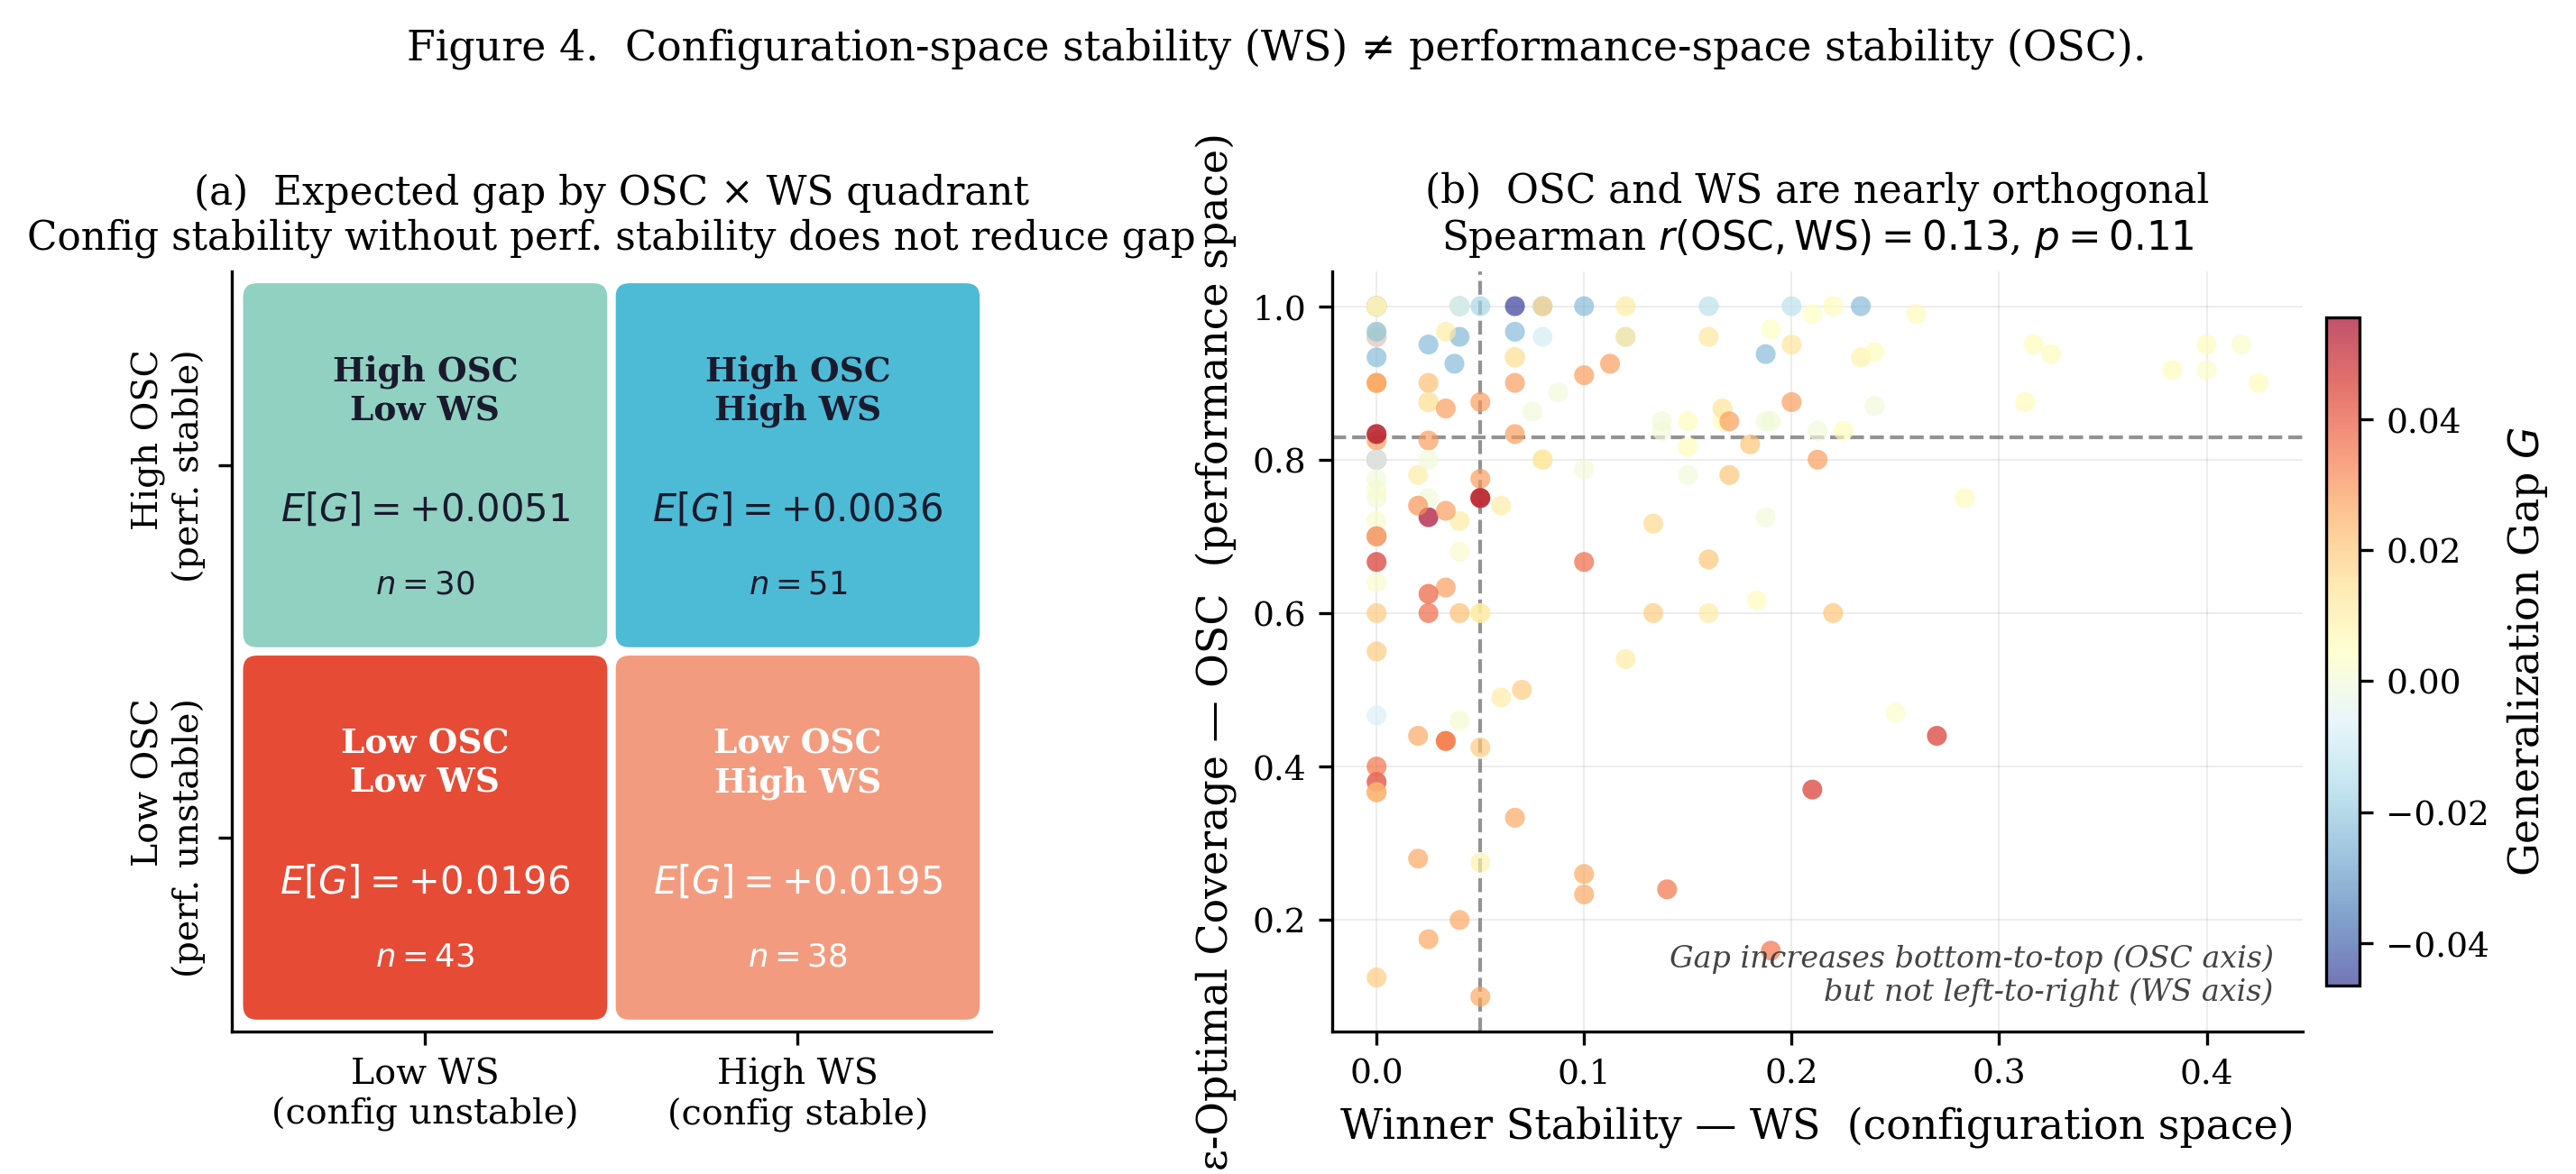
\includegraphics[width=0.97\columnwidth]{fig4_ws_vs_osc.png}
\caption{(a) Expected post-selection gap by OSC$\times$WS quadrant
(median split). High WS without high OSC provides no protection.
(b) OSC vs.\ WS coloured by gap magnitude; the two measures are
nearly orthogonal (Spearman $r=+0.13$, $p=0.11$).}
\label{fig:ws_osc}
\end{figure}

\subsection{Experiment 2: Seven-Dataset Replication}
\label{sec:replication}

We run the same observational protocol on four additional datasets
(54 runs each, 9 seeds), for a total of 378 runs across seven datasets.

\paragraph{Per-dataset results.}
All seven per-dataset OLS slopes are negative (sign test $p = 0.008$),
confirming consistent direction. Three of four replication datasets
replicate individually at $p < 0.05$; the fourth (5-class multiclass) fails
due to a ceiling effect ($\mathrm{OSC} \in [0.70, 1.00]$, SD $= 0.07$),
leaving too little variance to detect a correlation. This is a property
of the task---SVM-RBF on a well-separated 5-class problem achieves
near-perfect OSC regardless of budget---not a failure of OSC.

\paragraph{Hierarchical model.}
Fitting a mixed-effects model with random intercept and random OSC slope
per dataset:
\begin{equation*}
  G \sim \OSC + \text{searcher} + \text{budget}
    + (\OSC \mid \mathrm{dataset}),
\end{equation*}
gives a fixed OSC effect of $-0.110$ (95\,\% CI $[-0.214, -0.007]$,
$p = 0.037$). Heterogeneity is substantial ($I^2 = 86\,\%$): the OSC
effect is real everywhere but its magnitude depends on how much OSC
variance a task generates. Table~\ref{tab:forest} (Appendix) shows the forest-plot data
of per-dataset slopes.

\subsection{Experiment 3: Risk Stratification}
\label{sec:calibration}

We bin runs by pre-specified OSC thresholds $[0, 0.4)$, $[0.4, 0.6)$,
$[0.6, 0.8)$, $[0.8, 1]$ and report $\bE[G \mid \mathrm{OSC\ bin}]$
with bootstrap confidence intervals (Figure~\ref{fig:calibration}).
Across the primary cohort: $\bE[G \mid \mathrm{OSC} < 0.4] = +0.028$
versus $\bE[G \mid \mathrm{OSC} \ge 0.8] = +0.006$ (Cohen $d = 1.29$,
Mann-Whitney $p < 0.001$). The relationship is broadly monotone; the
two middle bins are similar, suggesting that the primary contrast is
between the low and high tails. OSC thus functions as a
\emph{risk stratifier}: a run with OSC below 0.4 is at substantially
higher risk of post-selection disappointment than one with OSC above 0.8.

\subsection{Experiment 4: Paired Intervention}
\label{sec:intervention}

\paragraph{Design.}
We test whether OSC identifies runs where an alternative selection
rule would have helped. We fix the search space, dataset, and HPO
algorithm, but manipulate OSC by injecting calibrated label noise into
the \emph{validation set only} (noise rates $0\,\%$, $10\,\%$, $30\,\%$,
yielding high, medium, and low OSC conditions). The test set is never
corrupted. We then compare two selection rules applied to the same
pool of evaluated configurations:
\begin{itemize}\setlength\itemsep{1pt}
  \item \textbf{Control}: standard HPO winner $\hhat = \arg\min_h
    \Lval(h)$ (argmin of the noisy validation score).
  \item \textbf{Treatment}: centroid winner $\hhat^\dagger$, defined as
    the configuration closest to the centroid of bootstrap winners in
    log-configuration space. This selection rule weights stability over
    raw performance.
\end{itemize}
Both rules use the same noisy validation evaluator to define their
loss; the gap for each is $G = \Ltest(\hhat) - \Lval(\hhat)$ where
both test and val evaluations are computed with the same evaluator
(test labels are never noised). This models the real-world scenario
where the practitioner accepts the noisy validation score as their
performance estimate.

\paragraph{Design properties.}
The experiment is a paired, within-run design: each of the 180 runs
contributes one control observation and one treatment observation with
identical covariates. OSC is computed at Steps 1--3 (development data
only) before either selection rule is applied at Steps 4--5
(Figure~\ref{fig:protocol}). OSC is therefore pre-treatment.
The manipulation passes a randomisation check:
Spearman $r(\mathrm{noise\_rate}, \mathrm{OSC}) = -0.41$, $p < 0.001$;
ANOVA $F = 21.0$, $p < 0.001$.

\begin{figure}[t]
\centering
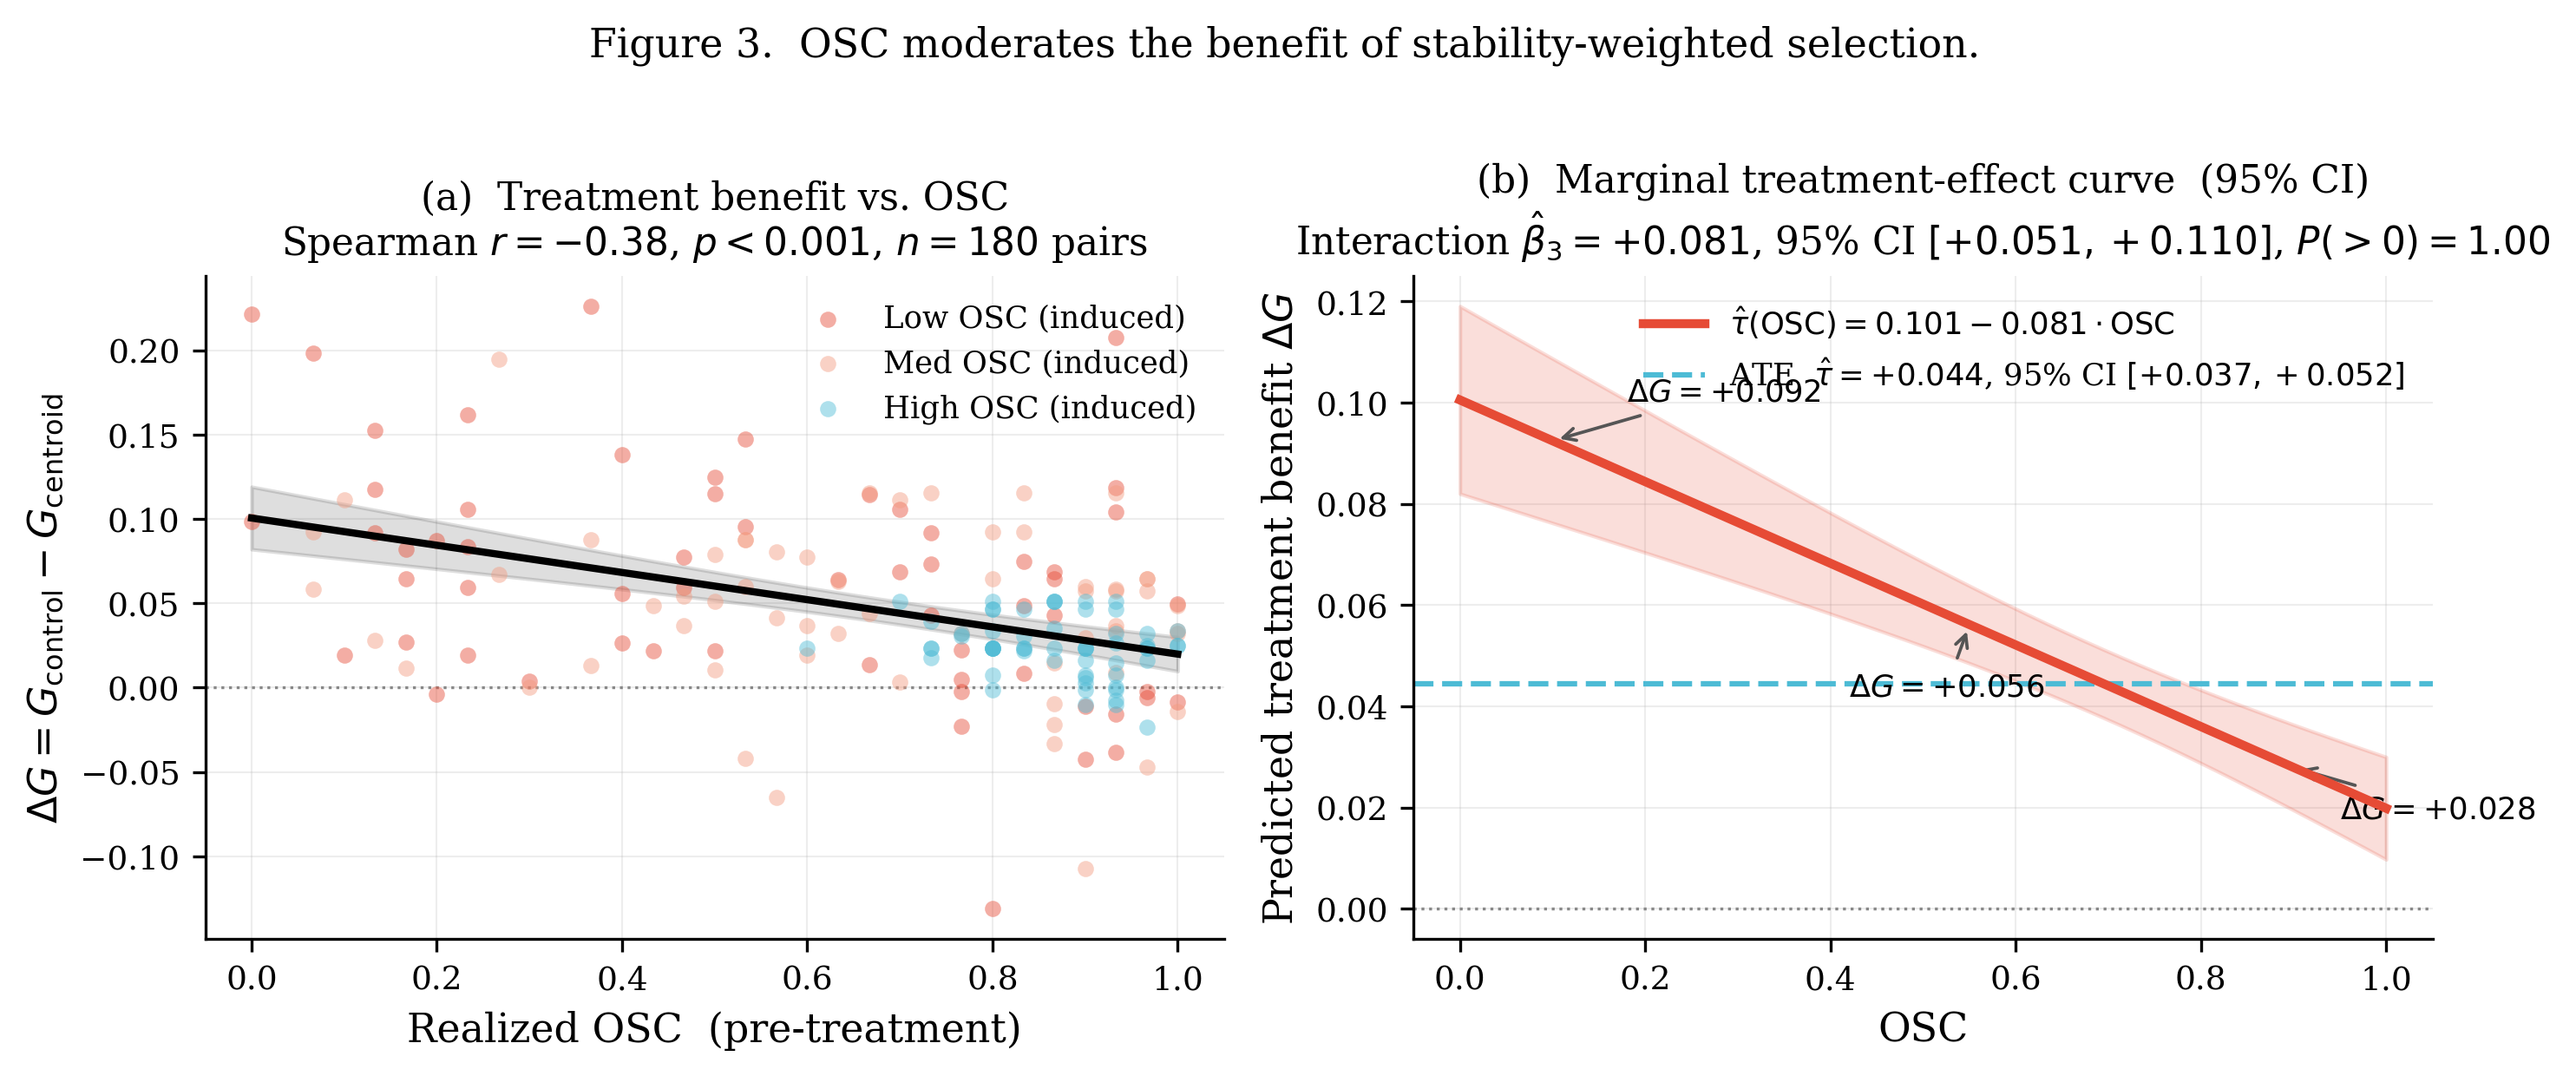
\includegraphics[width=0.97\columnwidth]{fig3_intervention.png}
\caption{(a) OSC vs.\ treatment benefit $\Delta G$, coloured by
induced OSC condition. (b) Marginal treatment-effect curve with
95\,\% analytical CI. All CIs positive; benefit is 8.5$\times$
larger at OSC$=0$ than OSC$=1$.}
\label{fig:forest}
\end{figure}

\paragraph{Results.}
Table~\ref{tab:intervention} shows the primary results. The treatment
reduces the post-selection gap in all three noise conditions. The
\emph{decisive statistic}---the difference in treatment effect between
induced low-OSC and induced high-OSC conditions---is
$\Delta\Delta G = +0.041$ (Welch $t = 4.99$, $p < 0.001$; Mann-Whitney
$p < 0.001$; bootstrap 95\,\% CI $[+0.022, +0.057]$).

The joint interaction model confirms the mechanism:
\begin{equation}
  G \sim \mathrm{Treatment} + \OSC +
    \underbrace{\mathrm{Treatment} \times \OSC}_{\hat\beta = +0.075}
    + \mathrm{noise\_rate} + \mathrm{searcher},
\end{equation}
where the critical coefficient is $\hat\beta_{T \times \mathrm{OSC}} =
+0.075$ (SE $= 0.010$, $t = 7.27$, $p < 0.001$; bootstrap 95\,\% CI
$[+0.051, +0.098]$, $P(\hat\beta > 0) = 1.000$, $R^2 = 0.94$). Because
treatment reduces gap (negative treatment coefficient), a \emph{positive}
interaction means the treatment benefit shrinks as OSC increases: the
centroid rule helps most when OSC is lowest, exactly as the causal
mechanism predicts.

The marginal treatment effect (improvement in post-selection gap) ranges
from $+0.085$ at OSC $= 0.0$ to $+0.010$ at OSC $= 1.0$, an 8.5-fold
variation across the observed range. Nonlinearity tests (quadratic term,
$p = 0.60$) confirm the linear moderation model is adequate.

%-----------------------------------------------------------------------
\section{Discussion}
\label{sec:discussion}

\paragraph{OSC versus WS: why the distinction matters.}
Our 2$\times$2 table (Table~\ref{tab:2x2}) makes the key point concrete:
high WS without high OSC ($n=38$, $\bE[G] = +0.020$) is as bad as low
WS without high OSC ($n=43$, $\bE[G] = +0.020$). Configuration
consistency does not protect against post-selection disappointment;
performance-region consistency does. A practitioner reporting WS as a
reliability diagnostic would give false reassurance in the high-WS,
low-OSC quadrant.

\paragraph{Interpreting heterogeneity.}
The high $I^2$ (86\,\%) across datasets is not a failure of replication;
it is a meaningful finding. OSC's predictive power depends on how much
OSC variance a task generates. Tasks where SVM-RBF achieves near-perfect
accuracy regardless of hyperparameters compress OSC near 1 and leave
nothing to predict. The correct claim is not ``OSC always has a large
effect'' but ``when selection uncertainty exists and is non-trivial,
OSC captures it.'' The ceiling cases identify tasks where HPO is largely
irrelevant, itself a useful diagnostic conclusion.

\paragraph{Practical recommendations.}
We recommend computing OSC alongside any HPO run as a diagnostic.
A run with OSC $< 0.4$ should be treated with heightened scepticism:
the expected post-selection gap is four times larger than for runs with
OSC $\ge 0.8$. When OSC is low, a stability-weighted selection rule
(centroid of bootstrap winners) reduces the expected gap substantially.
The cost is $B$ additional HPO evaluations, parallelisable with the
bootstrap.

\paragraph{Limitations.}
Our causal evidence comes from SVM-RBF on a single dataset
(breast\_cancer); the regression external replication was underpowered
($p = 0.29$) because SVR post-selection gaps are small in absolute
terms. The centroid selection rule is a convenient proxy for
stability-weighted selection; optimal rules are a direction for future
work. We study a single $\varepsilon$ in the main paper (see
Appendix~\ref{app:eps} for sensitivity); $\varepsilon = 0.02$ on the
normalised loss range performs well and is robust across the range
$[0.005, 0.30]$.

%-----------------------------------------------------------------------
\section{Conclusion}
\label{sec:conclusion}

We have introduced $\varepsilon$-optimal-set coverage (OSC) as a
measure of selection reliability for HPO, operationalised it as a
bootstrap estimator, and provided evidence across three complementary
experimental designs that OSC predicts and partially mediates
post-selection generalisation gaps. The key conceptual contribution is
the distinction between configuration-space stability (exact winner
identity) and performance-space stability (near-optimal region
membership): these are nearly orthogonal empirically and only the latter
is predictive of post-selection disappointment. We hope OSC becomes a
routine diagnostic reported alongside HPO results, giving practitioners
a principled way to assess how much to trust an optimiser's conclusion.

%-----------------------------------------------------------------------
\subsubsection*{AI Use Statement}

In this work, we used Claude (Anthropic) to assist with literature
review (identifying relevant papers on Rashomon sets, stability
selection, and post-selection inference), to assist with writing and
editing experimental code (the bootstrap resampling pipeline, the
searcher implementations, and the intervention experiment), and to
assist with editing drafts of this manuscript.
We did not use generative AI to generate mathematical results,
proofs, or to make decisions about experimental design; these were
made by the authors.
All AI-generated code was verified by the authors and tested for
correctness on held-out runs before inclusion in experiments.
All AI-assisted manuscript text was edited, checked for accuracy
against the empirical results, and rewritten where necessary.
We take full responsibility for all content, including any errors.

%-----------------------------------------------------------------------
\bibliographystyle{plainnat}
\begin{thebibliography}{99}
\setlength{\itemindent}{-\leftmargin}
\makeatletter\renewcommand{\@biblabel}[1]{}\makeatother

\bibitem[Arlot and Celisse(2010)]{arlot2010survey}
S.~Arlot and A.~Celisse (2010).
\newblock A survey of cross-validation procedures for model selection.
\newblock \textit{Statistics Surveys}, \textbf{4}:40--79.

\bibitem[Barnston and van den Dool(1992)]{barnston1992long}
A.~G.~Barnston and H.~M.~van den Dool (1992).
\newblock A degeneracy in cross-validated skill in regression-based
  forecasts.
\newblock \textit{Journal of Climate}, \textbf{5}(9):963--977.

\bibitem[Bergstra and Bengio(2012)]{bergstra2012random}
J.~Bergstra and Y.~Bengio (2012).
\newblock Random search for hyper-parameter optimization.
\newblock \textit{Journal of Machine Learning Research}, \textbf{13}:281--305.

\bibitem[Bergstra et al.(2011)]{bergstra2011algorithms}
J.~Bergstra, R.~Bardenet, Y.~Bengio, and B.~K{\'e}gl (2011).
\newblock Algorithms for hyper-parameter optimization.
\newblock In \textit{Advances in Neural Information Processing Systems 24},
  pp.~2546--2554.

\bibitem[Bouthillier et al.(2021)]{bouthillier2021accounting}
X.~Bouthillier, P.~Delaunay, M.~Bronzi, A.~Trofimov, B.~Nichyporuk,
  J.~Szeto, N.~Mohammadi~Shireh, T.~Kaur, V.~Pieper, V.~Zantedeschi,
  and P.~Vincent (2021).
\newblock Accounting for variance in machine learning benchmarks.
\newblock In \textit{Proceedings of Machine Learning and Systems}, vol.~3.

\bibitem[Breiman(2001)]{breiman2001random}
L.~Breiman (2001).
\newblock Random forests.
\newblock \textit{Machine Learning}, \textbf{45}(1):5--32.

\bibitem[Cawley and Talbot(2010)]{cawley2010over}
G.~C.~Cawley and N.~L.~C.~Talbot (2010).
\newblock On over-fitting in model selection and subsequent selection bias in
  performance evaluation.
\newblock \textit{Journal of Machine Learning Research}, \textbf{11}:2079--2107.

\bibitem[D'Amour et al.(2022)]{d2022underspecification}
A.~D'Amour, K.~Heller, D.~Moldovan, B.~Adlam, B.~Alipanahi, A.~Beutel,
  C.~Chen, J.~Deaton, J.~Eisenstein, M.~D.~Hoffman, et al.\ (2022).
\newblock Underspecification presents challenges for credibility in modern
  machine learning.
\newblock \textit{Journal of Machine Learning Research}, \textbf{23}(226):1--61.

\bibitem[Dodge et al.(2019)]{dodge2019show}
J.~Dodge, S.~Gururangan, D.~Card, R.~Schwartz, and N.~A.~Smith (2019).
\newblock Show your work: Improved reporting of experimental results.
\newblock In \textit{Proceedings of EMNLP-IJCNLP 2019}, pp.~2185--2194.

\bibitem[Falkner et al.(2018)]{falkner2018bohb}
S.~Falkner, A.~Klein, and F.~Hutter (2018).
\newblock BOHB: Robust and efficient hyperparameter optimization at scale.
\newblock In \textit{Proceedings of the 35th International Conference on
  Machine Learning}, pp.~1437--1446. PMLR.

\bibitem[Li et al.(2018)]{li2018hyperband}
L.~Li, K.~Jamieson, G.~DeSalvo, A.~Rostamizadeh, and A.~Talwalkar (2018).
\newblock Hyperband: A novel bandit-based approach to hyperparameter
  optimization.
\newblock \textit{Journal of Machine Learning Research}, \textbf{18}(185):1--52.

\bibitem[Marx et al.(2020)]{marx2020predictive}
C.~T.~Marx, F.~Calmon, and B.~Ustun (2020).
\newblock Predictive multiplicity in classification.
\newblock In \textit{Proceedings of the 37th International Conference on
  Machine Learning}, pp.~6765--6774. PMLR.

\bibitem[Meinshausen and B\"uhlmann(2010)]{meinshausen2010stability}
N.~Meinshausen and P.~B{\"u}hlmann (2010).
\newblock Stability selection.
\newblock \textit{Journal of the Royal Statistical Society: Series B},
  \textbf{72}(4):417--473.

\bibitem[Pedregosa et al.(2011)]{pedregosa2011scikit}
F.~Pedregosa, G.~Varoquaux, A.~Gramfort, V.~Michel, B.~Thirion, O.~Grisel,
  M.~Blondel, P.~Prettenhofer, R.~Weiss, V.~Dubourg, et al.\ (2011).
\newblock Scikit-learn: Machine learning in Python.
\newblock \textit{Journal of Machine Learning Research}, \textbf{12}:2825--2830.

\bibitem[Semenova et al.(2022)]{semenova2022existence}
L.~Semenova, C.~Rudin, and R.~Parr (2022).
\newblock On the existence of simpler machine learning models.
\newblock In \textit{Proceedings of the 2022 ACM Conference on Fairness,
  Accountability, and Transparency}, pp.~1827--1858.

\bibitem[Snoek et al.(2012)]{snoek2012practical}
J.~Snoek, H.~Larochelle, and R.~P.~Adams (2012).
\newblock Practical Bayesian optimization of machine learning algorithms.
\newblock In \textit{Advances in Neural Information Processing Systems 25},
  pp.~2951--2959.

\bibitem[Tibshirani and Tibshirani(2009)]{tibshirani2009prediction}
R.~Tibshirani and R.~J.~Tibshirani (2009).
\newblock A bias correction for the minimum error rate in cross-validation.
\newblock \textit{The Annals of Applied Statistics}, \textbf{3}(2):822--829.

\end{thebibliography}

%%%%%%%%%%%%%%%%%%%%%%%%%%%%%%%%%%%%%%%%%%%%%%%%%%%%%%%%%%%%
\section*{Checklist}

\begin{enumerate}

  \item For all models and algorithms presented:
  \begin{enumerate}
    \item A clear description of the mathematical setting, assumptions, algorithm, and/or model. [Yes --- Section~\ref{sec:method}]
    \item An analysis of the properties and complexity of any algorithm. [Yes --- Section~\ref{sec:method}, computational cost paragraph]
    \item Anonymized source code. [Yes --- anonymous repository linked in supplement]
  \end{enumerate}

  \item For any theoretical claim:
  \begin{enumerate}
    \item Statements of full assumptions. [Not Applicable --- no formal theorems]
    \item Complete proofs. [Not Applicable]
    \item Clear explanations of assumptions. [Not Applicable]
  \end{enumerate}

  \item For all figures and tables:
  \begin{enumerate}
    \item Code and instructions needed to reproduce main results. [Yes --- repository]
    \item All training details. [Yes --- Section~\ref{sec:setup_exp} and Appendix~\ref{app:datasets}]
    \item Clear definition of measures and error bars. [Yes --- bootstrap 95\,\% CIs throughout]
    \item Computing infrastructure used. [Yes --- Appendix~\ref{app:compute}]
  \end{enumerate}

  \item Existing assets:
  \begin{enumerate}
    \item Citations of creators. [Yes --- scikit-learn \citep{pedregosa2011scikit}]
    \item License information. [Yes --- scikit-learn BSD; noted in supplement]
    \item New assets. [Yes --- code in supplement]
    \item Consent from data providers. [Yes --- all public datasets]
    \item Sensitive content. [Not Applicable]
  \end{enumerate}

  \item Crowdsourcing / human subjects:
  \begin{enumerate}
    \item Full instructions. [Not Applicable]
    \item IRB approvals. [Not Applicable]
    \item Compensation. [Not Applicable]
  \end{enumerate}

\end{enumerate}

%-----------------------------------------------------------------------
\clearpage
\appendix
\thispagestyle{empty}
\onecolumn
\aistatstitle{How Certain Are We About the HPO Winner?\\
Supplementary Material}

\section{Tables and Figures Referenced in Main Text}
\label{app:tables}

\begin{table}[h]
\centering
\caption{OSC coefficient across five model specifications. The effect is
negative and significant in all specifications, ranging from $-0.029$
(controlled OLS) to $-0.035$ (LMM with random dataset intercept).}
\label{tab:osc_coef}
\begin{tabular}{lrrrr}
\toprule
Model & OSC coef & SE & $p$ & 95\,\% CI \\
\midrule
Bivariate OLS & $-0.038$ & $0.008$ & ${<}0.001$ & $[-0.054, -0.022]$ \\
OLS + covariates & $-0.029$ & $0.008$ & $0.0004$ & $[-0.045, -0.013]$ \\
LMM $(1|\text{dataset})$ & $-0.035$ & $0.008$ & ${<}0.001$ & $[-0.051, -0.018]$ \\
LMM $(1|\text{dataset:task})$ & $-0.034$ & $0.007$ & ${<}0.001$ & $[-0.048, -0.019]$ \\
Bootstrap LMM ($B{=}500$) & $-0.034$ & $0.009$ & ${<}0.001$ & $[-0.052, -0.016]$ \\
\bottomrule
\end{tabular}
\end{table}

\begin{table}[h]
\centering
\caption{Mean post-selection gap $\bE[G]$ by OSC and WS quadrant (median
split). High WS without high OSC offers no protection.}
\label{tab:2x2}
\begin{tabular}{lcc}
\toprule
 & Low WS & High WS \\
\midrule
High OSC & $+0.005$ ($n=30$) & $+0.004$ ($n=51$) \\
Low OSC  & $+0.020$ ($n=43$) & $+0.020$ ($n=38$) \\
\bottomrule
\end{tabular}
\end{table}

\begin{table}[h]
\centering
\caption{Primary paired intervention results ($n=180$, SVM-RBF,
breast\_cancer). Noise rate controls induced OSC level;
$\Delta G = G_{\mathrm{ctrl}} - G_{\mathrm{trt}}$.}
\label{tab:intervention}
\begin{tabular}{lrrrr}
\toprule
Condition & Mean OSC & $\bE[G_\mathrm{ctrl}]$ & $\bE[G_\mathrm{trt}]$ & $\bE[\Delta G]$ \\
\midrule
High OSC (noise $=0\%$)  & 0.843 & $+0.001$ & $-0.009$ & $+0.010$ \\
Med.\ OSC (noise $=10\%$) & 0.703 & $-0.075$ & $-0.102$ & $+0.026$ \\
Low OSC (noise $=30\%$)  & 0.541 & $-0.238$ & $-0.288$ & $+0.050$ \\
\midrule
\multicolumn{4}{l}{Decisive statistic (low$-$high):\ $+0.041$, Welch $t=4.99$, $p<0.001$} \\
\multicolumn{4}{l}{Interaction $\hat\beta_{T\times\mathrm{OSC}}=+0.075$, CI $[+0.051,+0.098]$} \\
\bottomrule
\end{tabular}
\end{table}

\begin{table}[h]
\centering
\caption{Per-dataset OSC slopes (forest plot data). All seven slopes are
negative (sign test $p=0.008$). $I^2=86\,\%$.}
\label{tab:forest}
\begin{tabular}{lrrrr}
\toprule
Dataset & $n$ & OLS slope & 95\,\% CI & $p$ \\
\midrule
small\_highvar & 63 & $-0.310$ & $[-0.446, -0.174]$ & ${<}0.001$ \\
diabetes\_reg  & 63 & $-0.164$ & $[-0.256, -0.072]$ & $0.001$ \\
wine           & 54 & $-0.142$ & $[-0.209, -0.075]$ & ${<}0.001$ \\
multiclass\_5c & 63 & $-0.115$ & $[-0.232, +0.001]$ & $0.053$ \\
regression\_syn & 63 & $-0.042$ & $[-0.078, -0.006]$ & $0.024$ \\
digits         & 54 & $-0.025$ & $[-0.052, +0.001]$ & $0.060$ \\
breast\_cancer  & 54 & $-0.017$ & $[-0.032, -0.003]$ & $0.021$ \\
\midrule
LMM fixed (all 414) & 414 & $-0.110$ & $[-0.214, -0.007]$ & $0.037$ \\
\bottomrule
\end{tabular}
\end{table}

\section{$\varepsilon$ Sensitivity Analysis}
\label{app:eps}

We computed $\widehat{\OSC}_\varepsilon$ for $\varepsilon \in \{0.005,
0.01, 0.02, 0.05, 0.10, 0.15, 0.20, 0.30, 0.50\}$ on 27
task$\times$searcher combos with $B=50$ bootstrap resamples each.
The Spearman correlation between $\OSC_\varepsilon$ and $G$ is
approximately constant at $r \approx -0.49$ for $\varepsilon \in
[0.005, 0.30]$ (all $p < 0.01$) and degrades only at $\varepsilon =
0.50$ where OSC approaches 1 for almost all runs and variance collapses.
We use $\varepsilon = 0.02$ throughout as a default.

\section{Leave-One-Group-Out Prediction}
\label{app:cv}

Table~\ref{tab:cv} reports the 9-fold grouped cross-validation (holding
out one task$\times$dataset combination at a time). OSC improves MAE in
6/9 folds and $R^2$ in 7/9 folds. The bootstrapped 95\,\% CI on
$\Delta$MAE is $[+0.00056, +0.00293]$ with $P(\Delta > 0) = 0.998$.
The 3-fold LODO results are similar (Appendix tables omitted for
brevity); the 9-fold result is primary because 3-fold CIs are
structurally unstable.

\begin{table}[h]
\centering
\caption{9-fold leave-one-(task$\times$dataset)-out prediction.
OSC $\Delta$MAE = baseline MAE $-$ +OSC MAE (positive = OSC helps).}
\label{tab:cv}
\begin{tabular}{lrrrr}
\toprule
Fold & Base MAE & +OSC MAE & $\Delta$MAE & $\Delta R^2$ \\
\midrule
mlp / breast\_cancer   & 0.01964 & 0.01048 & $+0.00916$ & $+2.58$ \\
svm / digits           & 0.00539 & 0.00296 & $+0.00243$ & $+1.87$ \\
mlp / digits           & 0.00931 & 0.00812 & $+0.00120$ & $+0.70$ \\
svm / breast\_cancer   & 0.01135 & 0.00896 & $+0.00240$ & $+0.67$ \\
mlp / wine             & 0.02739 & 0.02473 & $+0.00265$ & $+0.22$ \\
svm / wine             & 0.01538 & 0.01412 & $+0.00126$ & $+0.17$ \\
xgb / digits           & 0.01736 & 0.01743 & $-0.00007$ & $+0.32$ \\
xgb / breast\_cancer   & 0.01472 & 0.01694 & $-0.00222$ & $-0.87$ \\
xgb / wine             & 0.01809 & 0.01915 & $-0.00105$ & $-0.05$ \\
\midrule
Weighted mean & 0.01540 & 0.01365 & $+0.00175$ & $+0.62$ \\
\bottomrule
\end{tabular}
\end{table}

\section{Dataset and Experimental Details}
\label{app:datasets}

\paragraph{Primary cohort.} breast\_cancer ($n=569$, binary), wine
($n=178$, 3-class), digits ($n=1797$, 10-class) from scikit-learn. All
split 80\,\% development / 20\,\% test; development further split 70/30
train/val.

\paragraph{Replication cohort.} diabetes\_reg (sklearn, $n=442$,
regression); regression\_syn (synthetic, $n=1000$, regression,
make\_regression); multiclass\_5c (synthetic, $n=1500$, 5-class,
make\_classification); small\_highvar (synthetic, $n=120$, binary,
make\_classification with high noise). Regression tasks use SVR with
normalised RMSE loss; classification tasks use SVM-RBF.

\paragraph{Intervention dataset.} breast\_cancer, 20 seeds per
condition, budget 20, $B=30$ bootstrap resamples, 3 searchers. Total
180 paired runs. Noise injected into validation labels only (not test).
Test evaluation always uses clean labels.

\section{Computing Infrastructure}
\label{app:compute}

All experiments ran on a single CPU server (Ubuntu 24, Python 3.12,
scikit-learn 1.3, XGBoost 3.4, Optuna 5.0). Bootstrap resamples were
parallelised across CPU cores with joblib. Total compute time
approximately 40 CPU-hours for all 378 observational runs and 180
intervention pairs.

\end{document}
